\chapter{Guidance and path generation}

The CCPP methods described in the previous chapter generate only one waypoint ahead in time. The next waypoint is determined only after the USV has reached its current waypoint. This motivates an online feasible path generation strategy. Upon each new waypoint, a feasible path is generated from the current USV pose to the next waypoint. A distinction is made here between path planning, as the generation of waypoints, and path generation, as the generation of a smooth curve between two points. To ensure that this curve is feasible, the USV's turning radius and speed must be taken into account. Given the curve from the path generation strategy, a guidance law generates continuous course and speed control that is passed on to the USV's onboard system.  

\section{Feasible path generation using straight lines and arc segments} \label{sec:pathgen}

A simple Dubins path consists of an arc segment followed by a straight line. This path is the shortest path that can be generated from a configuration (position and heading) to a position \citep{Scibilia2012}. Given the initial position and heading $p_q = (x_q, y_q)$ and $\theta_q$ and the final position $p_n$, the aim is to find the shortest path from $p_q$ to $p_n$ with initial heading $\theta_q$. Furthermore, the turning radius $\rho$ of the arc segment must be greater than the minimum feasible turning radius of the USV, i.e. $\rho \geq \rho_{min}$, where $\rho_{min}$ is the turning radius at the minimum required operating speed of the USV. The turning radius $\rho$ is a design parameter.

%If the minimum feasible turning radius of the USV, $\rho_{min}$, is smaller than half the distance between the start and end point, i.e. $\rho_{min} < \frac{|p_q - p_n|}{2}$, a simple Dubins path can be constructed. This places a constraint on the distance between subsequent waypoints generated by the CCPP method

\subsection{Turning direction}

Consider the straight line defined by the initial position and heading. The distance from $p_n$ to this line is given by 
\begin{equation}
	e_{nq} = -[x_n - x_q]\sin(\theta_q) + [y_n - y_q]\cos(\theta_q).
\end{equation}
The turning direction $\delta$ can be determined checking the sign of $e_{nq}$, 
\begin{equation}
\delta = 
\begin{cases}
1, & \text{if } e_{nq} > 0 \\
-1, & \text{otherwise.}
\end{cases}
\end{equation}
The value $\delta = 1$ corresponds to a left turn, and $\delta = -1$ corresponds to a right turn (z-axis assumed positive upward).

\subsection{Center of turning circle}

The arc segment is a segment of a turning circle which is located on a line perpendicular to the heading line and that goes through $p_q$. The coordinates for the center of the turning circle are given by
\begin{equation}
p_c = (x_c, y_c) = 
\begin{cases}
(x_q + \sin(\theta_q)\rho, y_q - \cos(\theta_q)\rho), & \text{if it is a right turn}  \\
(x_q - \sin(\theta_q)\rho, y_q + \cos(\theta_q)\rho), & \text{if it is a left turn,} 
\end{cases}
\end{equation}
and the circle has a radius $\rho$. In order for a Simple Dubins path to be constructed, the turning radius $\rho$ must be small enough such that the final position $p_n$ is not located inside the turning circle. Ensuring that the turning radius $\rho$ is smaller than half the distance between the start and end point, i.e. $\rho_{min} < \frac{|p_q - p_n|}{2}$, is a sufficient condition that can be imposed by properly choosing the distance between waypoints in the CCPP methods.

\subsection{Tangent point}

The arc segment starts in $p_q$ and follows the turning circle in the turning direction. The end point of the arc segment, however, is still unknown. This is determined by one of the tangent points generated by the tangent lines from the final position $p_n$ to the circle. The two lines tangent to the turning circle can be found by geometrical considerations, for instance by solving the second order trigonometric equation \citep{Scibilia2012}
\begin{equation}
((x_c - x_n)\sin(\beta) + (y_n - y_c)\cos{\beta})^2 = \rho^2,
\end{equation}
where $\beta$ is the angle of the tangent line. From this, two tangent points are obtained, and the first one encountered along the direction of rotation is used as the endpoint of the arc segment, denoted $p_l$. The geometry of the Simple Dubins path is shown in \figref{fig:dubins_ex}.

\begin{figure}[h!]
	\centering
	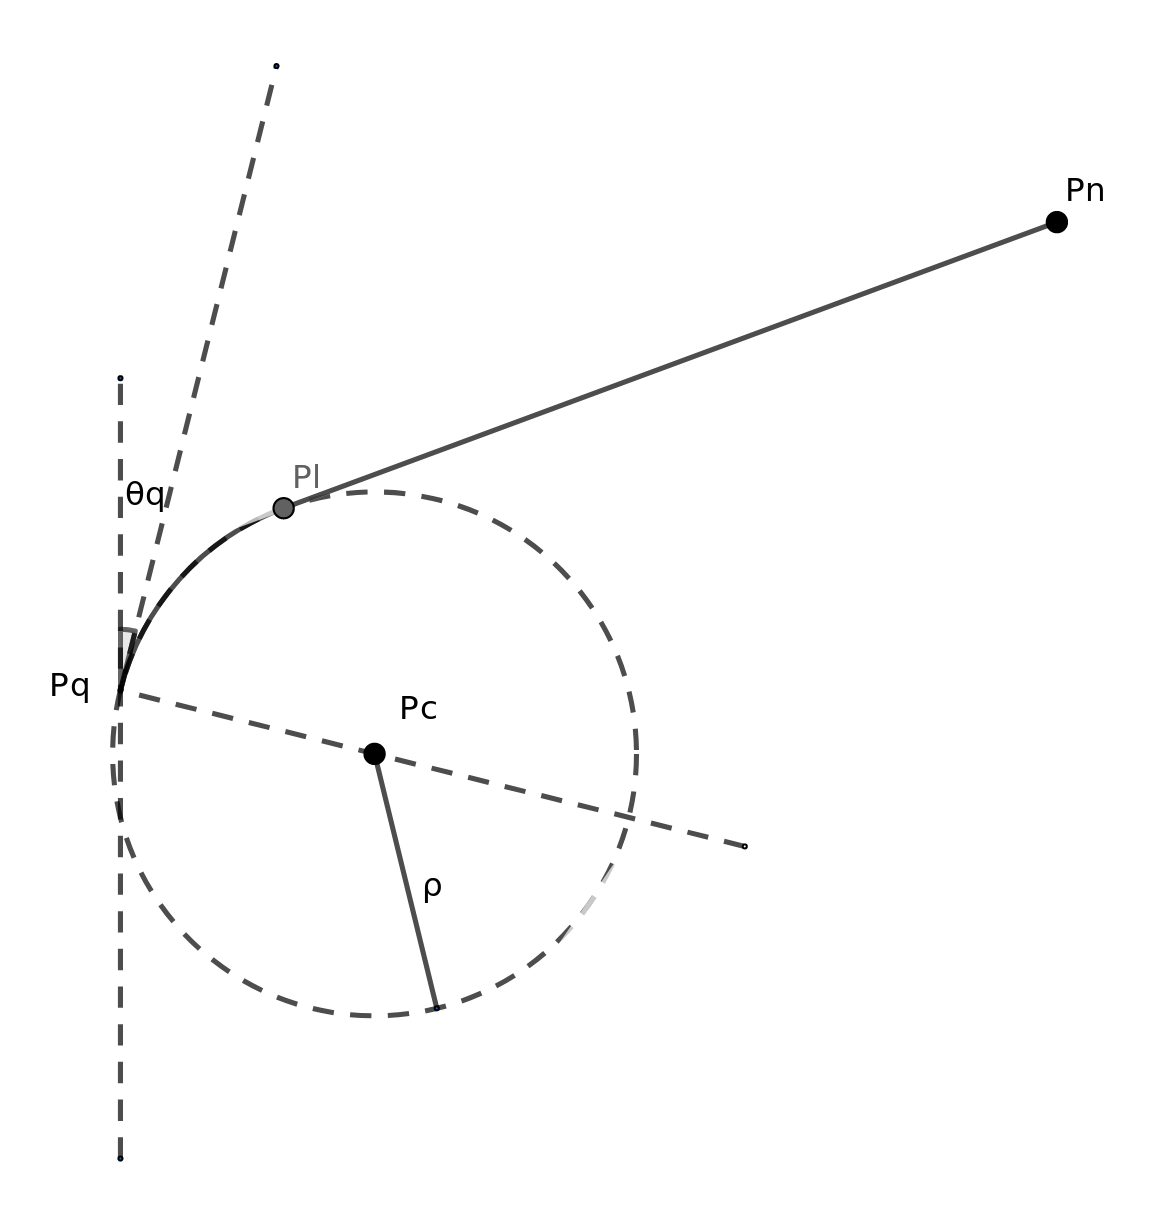
\includegraphics[width=0.5\textwidth]{fig/guidance/dubins}
	\caption{Simple Dubins path geometry.}
	\label{fig:dubins_ex}
\end{figure}

\subsection{Generating the path}

In ROS, a path is described by a \path{nav_msgs/Path} message, which consists of an array of poses. Now that the turning direction, turning circle and tangent point are known, generating poses on the path is trivial. The final heading of the path becomes
\begin{align}
	\theta_n = \text{atan2}(y_n - y_l, x_n - x_l)
\end{align}
where atan2 is a generalization of arctan that also determines the correct quadrant. The resolution of the generated path in the implemented system, i.e. the distance between consecutive poses, is determined by a user-specified parameter. A simple Dubins path can be seen in \figref{fig:dubins_rviz}.

\begin{figure}[h!]
	\centering
	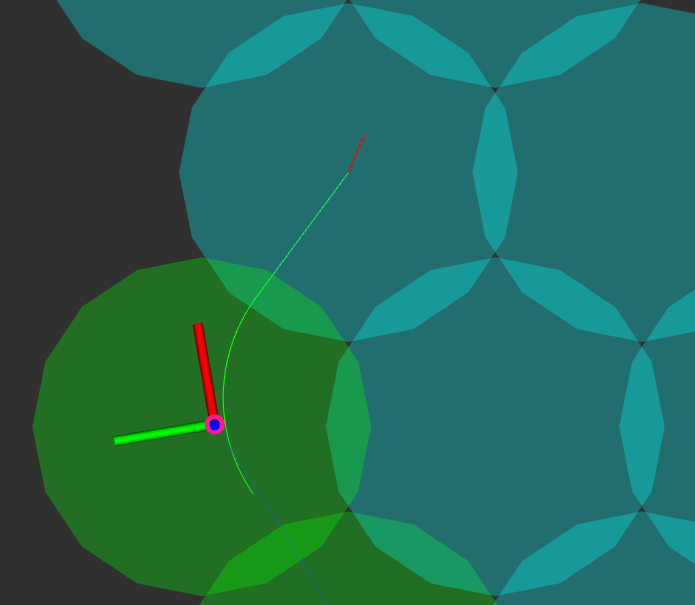
\includegraphics[width=0.5\textwidth]{fig/guidance/dubins-path}
	\caption{A generated simple Dubins path (green curve).}
	\label{fig:dubins_rviz}
\end{figure}



\section{Curved path line-of-sight guidance law with time-varying lookahead distance}

The guidance law will keep the USV on the path, or lead it towards the path if the position error is nonzero. The input to the guidance law is the path generated in Section \ref{sec:pathgen}, and the outputs are speed and course assignments. \figref{fig:los-geometry} shows the geometry of the curved path LOS guidance problem and some of the variables involved. The method presented in this section is based on \citet{lekkas2014integral}. 

\begin{figure}[h!]
	\centering
	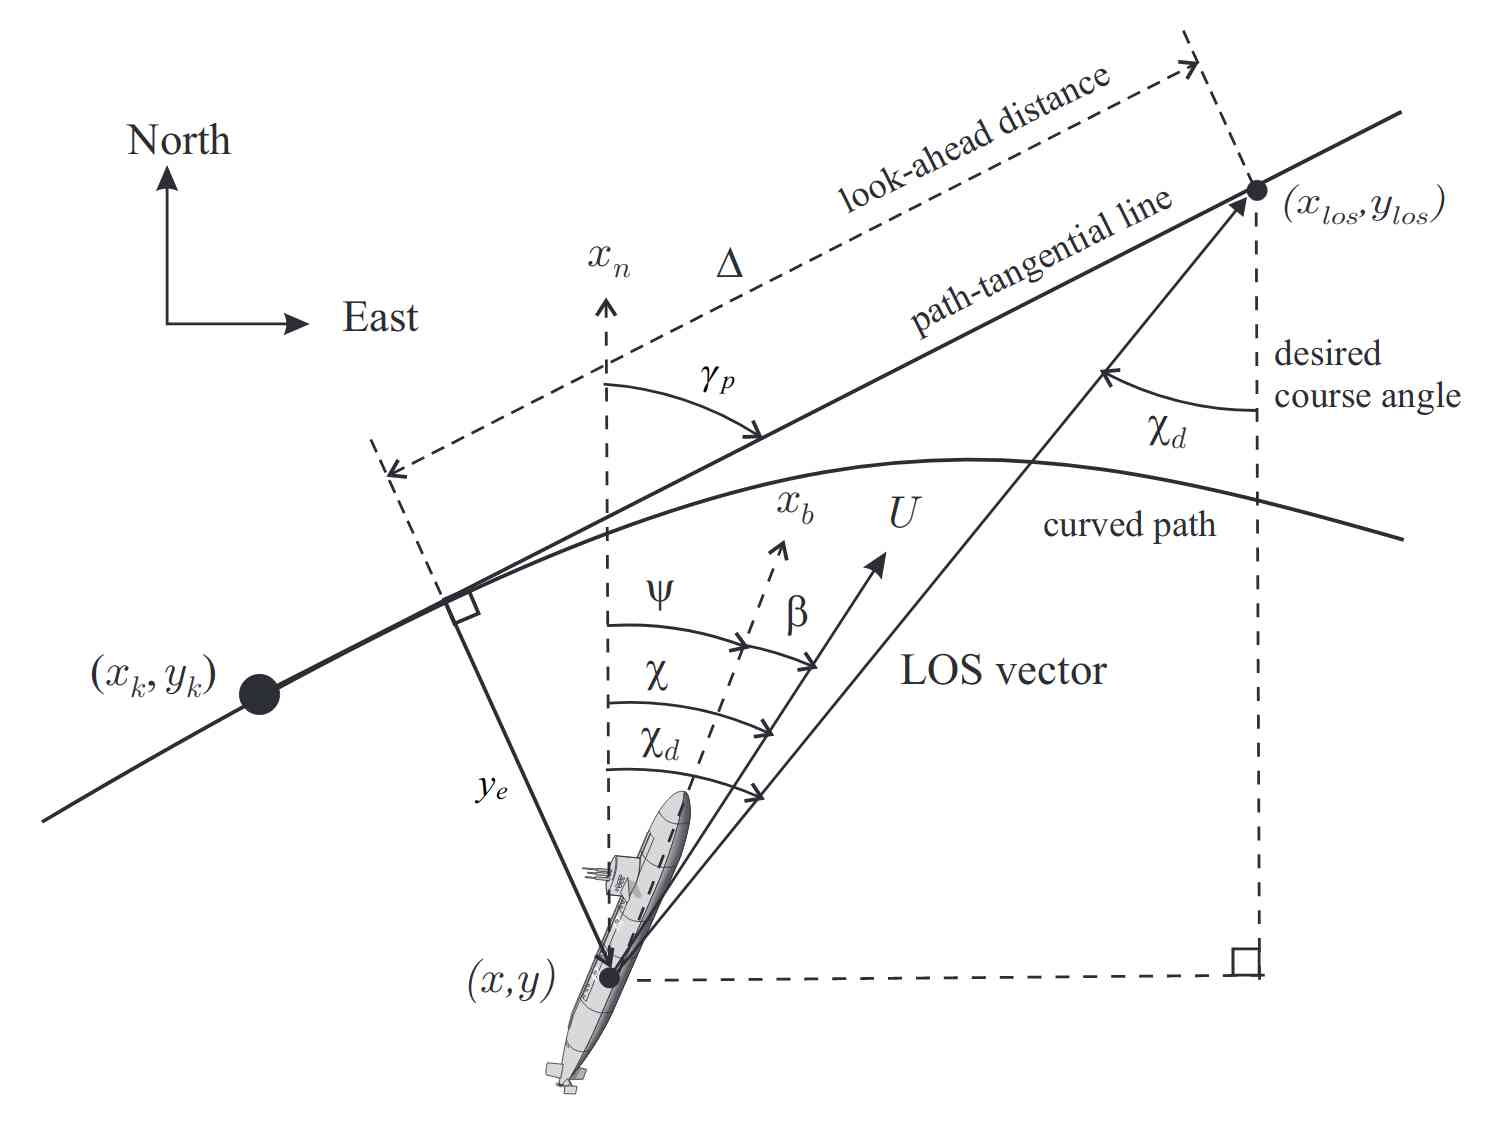
\includegraphics[width=0.7\textwidth]{fig/guidance/curved-guidance.jpg}
	\caption[Line-of-sight guidance geometry for curved paths.]{Line-of-sight guidance geometry for curved paths \citep{lekkas2014integral}.}
	\label{fig:los-geometry}
\end{figure}

\subsection{Cross-track error}

The cross-track error is the orthogonal distance from the USV position $(x,y)$ to a path-tangential reference frame defined by a point $(x_p,y_p)$ and rotated an angle $\gamma_p$ about the z-axis. The point $(x_p, y_p)$ is the point on the path that is closest to the USV position
\begin{equation}
(x_p,y_p,\theta_p) = \argmin_{(x_i,y_i,\theta_i) \ \in \ P} \sqrt{(x_i - x)^2 + (y_i - y)^2}
\end{equation} 
where $P = [(x_1,y_1,\theta_1), (x_2,y_2,\theta_2), ... , (x_n,y_n,\theta_n)]$ is the path, and $n$ is the number of poses in the path. The path tangential angle at any point on the path is then given by $\gamma_p = \theta_p$. The cross-track error can be computed by
\begin{equation}
y_e = -(x - x_p)\sin(\gamma_p) + (y - y_p)\cos(\gamma_p).
\end{equation}
The control objective for curved path following then becomes
\begin{equation}
\lim_{t \to +\infty} y_e(t) = 0.
\end{equation}

\subsection{Guidance law}

An LOS vector is constructed from the USV to a point $(x_{los}, y_{los})$ located on the path-tangential line. The distance from the closest point on the path $(x_p,y_p)$ to $(x_{los},y_{los})$ depends on a lookahead distance $\Delta(t) > 0$. From geometric consideration of \figref{fig:los-geometry}, the guidance law is given by
\begin{equation} \label{eq:guidance_law}
\chi_d = \gamma_p + \text{arctan}\left( \frac{-y_e}{\Delta} \right)
\end{equation}
where $\chi_d$ is the desired course angle of the USV defined as
\begin{equation}
\chi_d = \psi_d + \beta.
\end{equation} 
$\psi_d$ is the desired heading angle and $\beta$ is the sideslip angle. Sideslip is the deviation between where the USV is looking (heading), and the direction it is moving (course). It is caused by a nonzero sway velocity component, and occurs due to external forces such as currents, or lateral accelerations while turning. Since the Otter USV's onboard system uses course control, this is already compensated for.

\subsection{Time-varying lookahead distance} 

From \figref{fig:los-geometry} it is easy to see that a small lookahead distance results in a more aggressive steering, i.e. the desired path is reached faster. However, it will also contribute to unwanted oscillations around the path. A large lookahead distance produces smoother steering which avoids oscillations, but it also means that it takes longer to converge to the path. This motivates the use of a time-varying lookahead distance. By implementing a time-varying lookahead distance, the goal is to keep both the advantage of a faster convergence rate, and the reduction in unwanted oscillations. \citet{lekkas2014integral} proposes the following formula
\begin{equation} \label{eq:delta}
\Delta(y_e) = (\Delta_{max} - \Delta_{min}) e^{-K_\Delta y_e^2} + \Delta_{min}
\end{equation} 
where $\Delta_{max}$ and $\Delta_{min}$ are the maximum and minimum values for $\Delta$. The convergence rate $K_\Delta$, along with $\Delta_{max}$ and $\Delta_{min}$ constitute design parameters to be set by the user. 

\eqref{eq:delta} works by assigning a small value to $\Delta$ when the USV is far from the desired path, and a large value when it is close to the path. Since a small $\Delta$ results in aggressive steering, the USV will quickly converge towards the path when it is far away. Similarly, when the USV close to the path, a large $\Delta$ results in smoother steering which gives smaller overshoot and fewer oscillations. As opposed to a constant lookahead distance $\Delta$, \eqref{eq:delta} increases the number of design parameters that must be determined by the user.

\subsection{Speed assignment}

The following speed assignment is proposed
\begin{equation}
U_d = \max(U_{max} * (1 - \frac{|y_e|}{y_{max}} - \frac{|\tilde{\chi}|}{\chi_{max}}) + U_{min}, U_{min})
\end{equation}
where $U_d$ is the desired speed, $U_{max}$ and $U_{min}$ are the upper and lower limits for the speed, $y_e$ is the cross-track error, and $\tilde{\chi} = \chi - \chi_d$ is the error in the course angle. $y_{max}$ and $\chi_{max}$ are design parameters for the maximum allowed cross-track error and course angle error before the speed is assigned its minimum possible value.

This speed assignment ensures that the speed is lowered when the USV deviates from its path. With a lower speed the turning radius decreases, which in turn makes it easier for the USV to get back on the desired path. When the speed reaches its minimum, i.e. $U = U_{min}$, the USV will achieve its minimum turning radius $\rho_{min}$ which ensures that any generated path can be followed. An additional benefit is that when the USV tracks the path well, the speed is increased in order to save time.

\subsection{Interfacing with the Otter USV's thrusters}

The guidance system must be connected to the Otter USV's onboard system, since the onboard system already contains the thrust allocation strategies and low-level controllers required to steer the USV. The onboard system has therefore been modified to accept speed and course assignments over UDP. Similarly, the guidance system is extended to send these messages. The messages are serialized based on Google's Protocol Buffers \citep{wiki:protobuf}, which is a simple and effective way of communicating between different systems.

Before the messages can be sent, however, the desired course angle in the SLAM map's coordinate frame must be converted to an angle in the NED frame. The difference between the coordinate frames is just an offset, and can be adjusted for as follows
\begin{equation}
\chi_d = \chi_d^{SLAM} - \chi^{SLAM} + \chi 
\end{equation}
where $\chi$ and $\chi_d$ are the course and desired course angle in NED, and $\chi^{SLAM}$ and $\chi_d^{SLAM}$ are the course and desired course angle in the SLAM map's coordinate frame.
